%%%%%%%%%%%%%%%%%%%%%%%%%%%%%%%%%%%%%%%%%%%%%%%%%%%%%%%%%%%%%%%%%
%_____________ ___    _____  __      __ 
%\____    /   |   \  /  _  \/  \    /  \  Institute of Applied
%  /     /    ~    \/  /_\  \   \/\/   /  Psychology
% /     /\    Y    /    |    \        /   Zuercher Hochschule 
%/_______ \___|_  /\____|__  /\__/\  /    fuer Angewandte Wissen.
%        \/     \/         \/      \/                           
%%%%%%%%%%%%%%%%%%%%%%%%%%%%%%%%%%%%%%%%%%%%%%%%%%%%%%%%%%%%%%%%%
%
% Project     : Seminararbeit
% Title       : 
% File        : einfluss.tex Rev. 00
% Date        : 10.10.2012
% Author      : Till J. Ernst
%
%%%%%%%%%%%%%%%%%%%%%%%%%%%%%%%%%%%%%%%%%%%%%%%%%%%%%%%%%%%%%%%%%
\thispagestyle{empty}
\chapter{Einfluss Sozialer Medien auf das Subjektive Wohlbefinden}\label{chap.einfluss}
\glsresetall
In diesem Kapitel wird der Einfluss erläutert, wie sich \gls{sm} auf das \gls{swb} auswirken. Dazu werden verschieden Studien untersucht und mittels Concept Map grafisch zusammengeführt. Der Einfluss auf das \gls{swb} ist von verschiedenen Faktoren abhängig, welche in Abbildung~\ref{fig.ConceptMapSwbSm} ersichtlich sind (eine grössere Darstellung ist im Anhang \ref{sec.anhangGrafik} zu finden).
%Abbildung von ConceptMap SWB und SM
\begin{figure}[h]
	\centering
		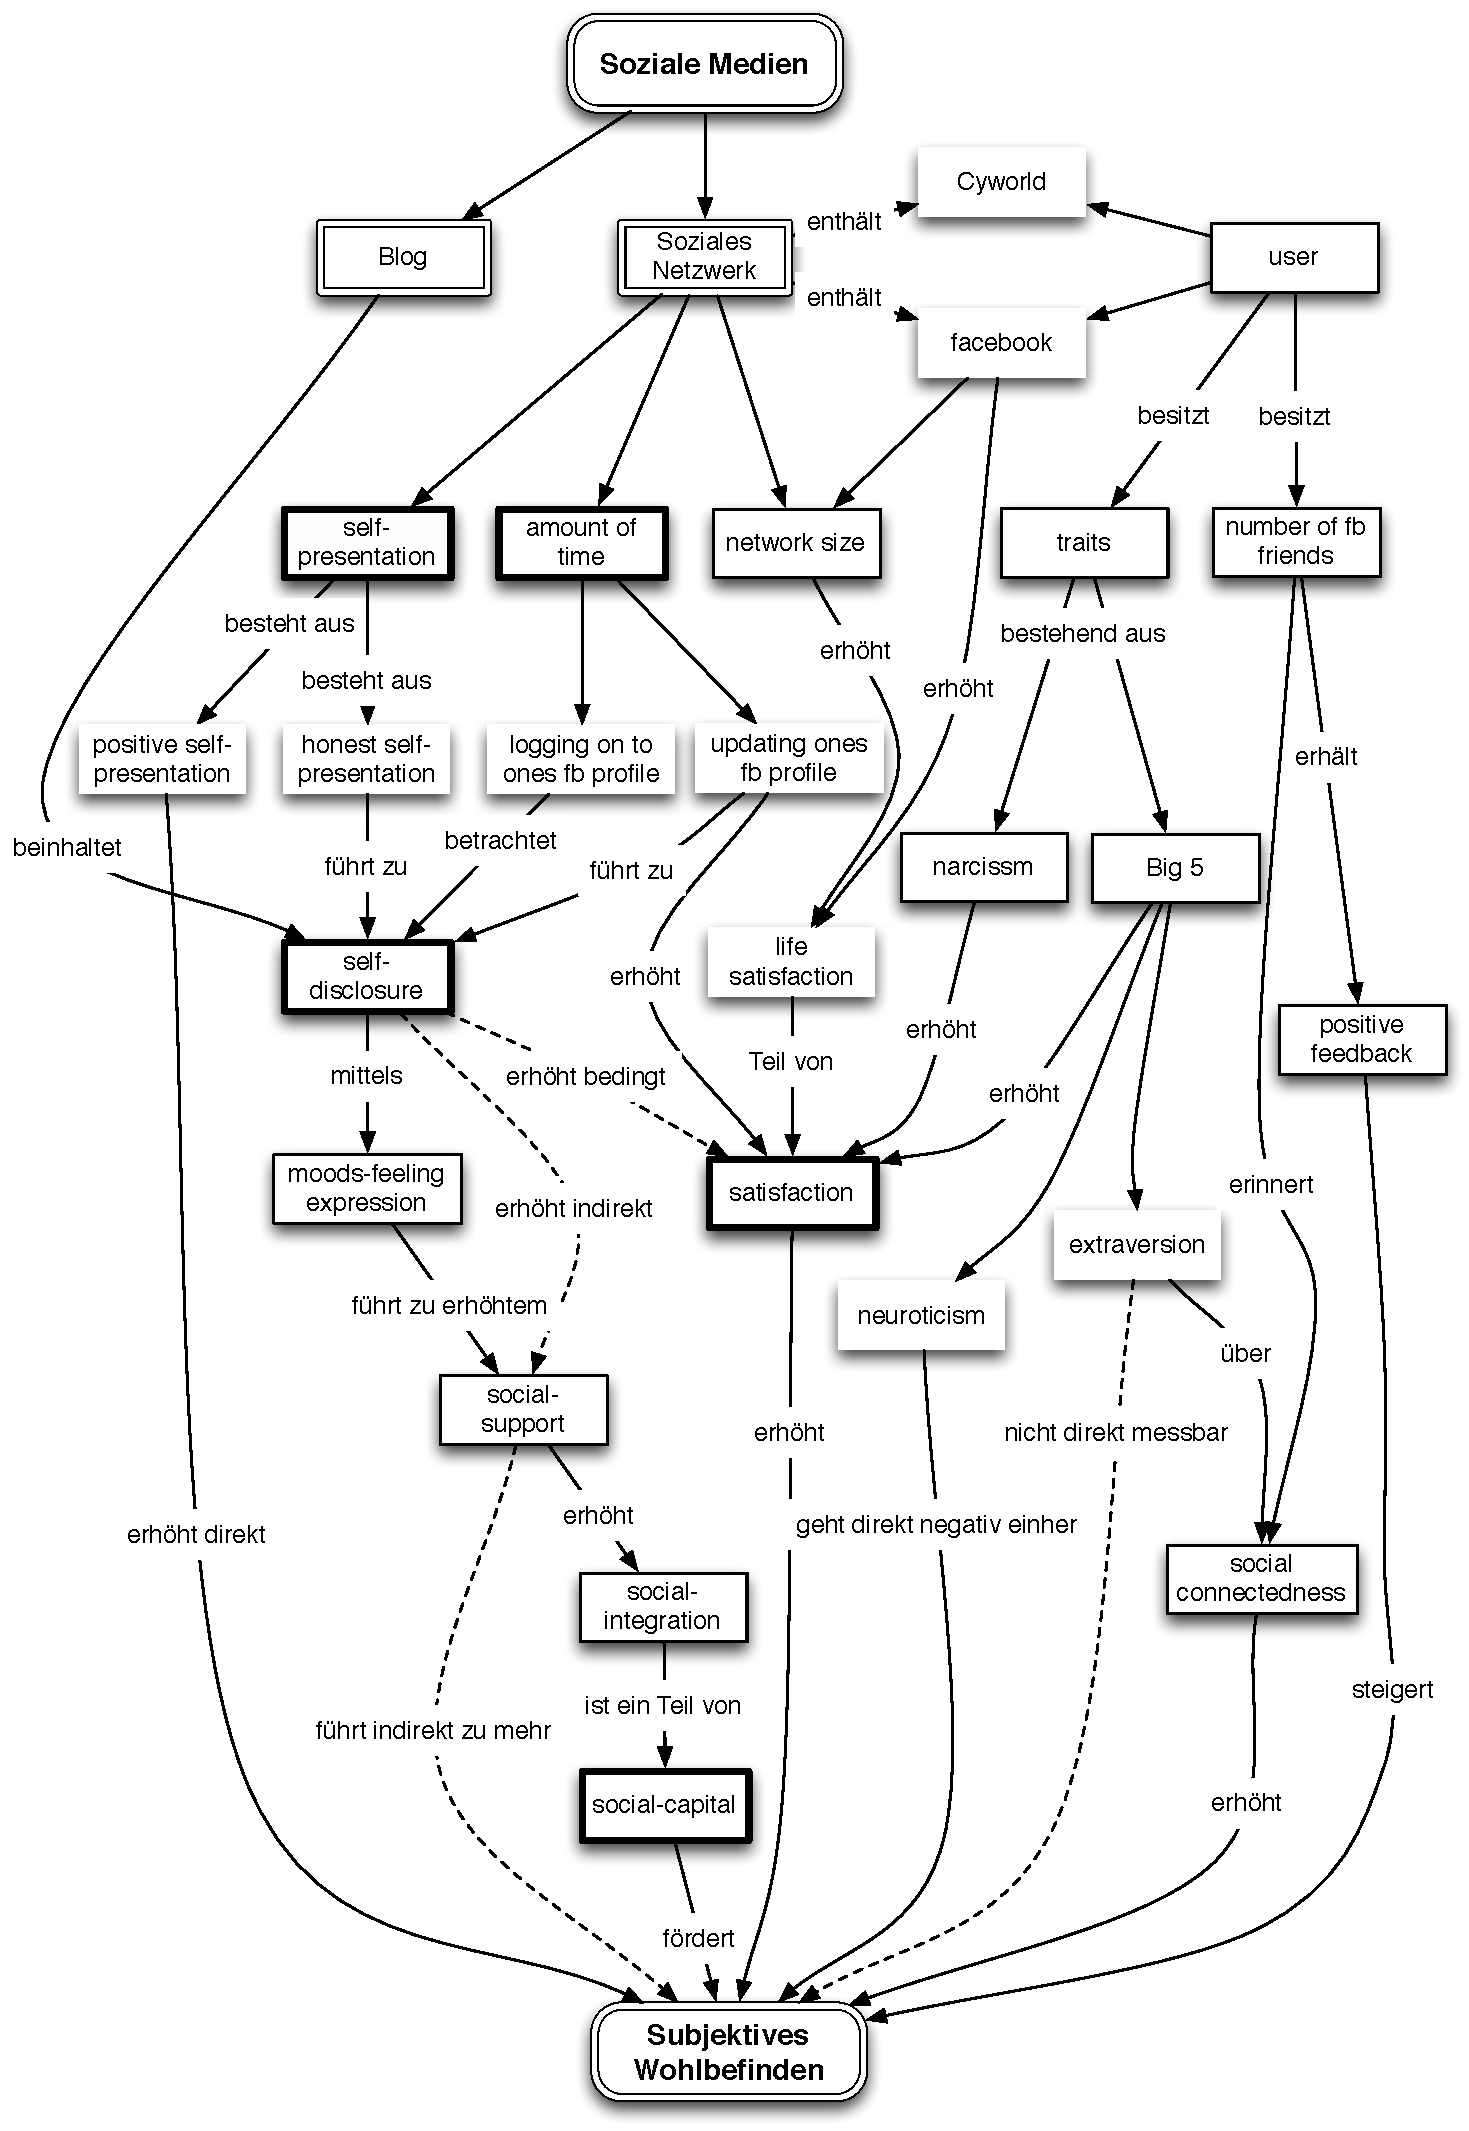
\includegraphics[width=0.4\textwidth]{images/grafiken/conceptMap_Swb_Sm_v2.pdf}
	\caption{ConceptMap - Subjektives Wohlbefinden und Soziale Medien}
	\label{fig.ConceptMapSwbSm}
\end{figure} \newline
Die Grafik stellt einen Zusammenzug unterschiedlicher Studien dar, die sich mit den Auswirkungen von \gls{sm} auf das \gls{swb} auseinander setzen. Darin sind die verschiedenen Konstrukte ersichtlich, die in den Studien verwendet wurden. Gelesen wird die Grafik ausgehend von den \gls{sm} entlang den Verbindungslinien bis hin zum \gls{swb}.\newline
Innerhalb der Grafik wurden die Englischen Begriffe aus den Studien übernommen. Bei den Verbindungslinien wurde mit Deutschen Wörtern gearbeitet.\newline
In den folgenden Unterkapiteln werden diese Konzepte anhand der Grafik erläutert. Dazu wird die Grafik in verschiedene Stränge unterteilt, um den komplexen Informationsgehalt in übersichtliche Häppchen aufzuteilen. Die Stränge sollen von den \gls{sm} ausgehend, über wichtige Konzepte und Begriffe, bis hin zum \gls{swb} führen. Da es sich um eine komplexe Thematik handelt, ist es nicht immer möglich die Grenzen scharf zu ziehen. Viele Konzepte überschneiden sich und greifen ineinander über.\newline 
Die in der Grafik markierten Konzepte und Begriffe werden in den folgenden Kapiteln näher erläutert. Wo dies möglich ist, werden die englischen Begriffe ins Deutsche übersetzt. Für Begriffe, bei denen die ursprüngliche Bedeutung durch einen unsachgemässe Übersetzung gefährdet ist, oder das deutsche Pendant dazu fehlt oder unklar ist, wird das originale englische Wort verwendet. Bei den jeweiligen Worterklärungen wird dem Englischen Begriff eine mögliche Deutsche Übersetzung mitgeliefert, wobei hier zu beachten ist, dass die Begriffe in den Studien nicht immer identisch verwendet werden und die Bedeutung je nach Verwendung des Autors leicht abweichen kann.

%UK Self-Presentation, Self-dicslosure und social capital
%----------------------------------------------------------------------
\section{Selbstdarstellung, Selbstoffenbarung und Soziales Kapital}\label{sub.selfp}
In diesem Kapitel wird auf den Einfluss von Selbstdarstellung, Selbstoffenbarung und Soziales Kapital als Haupteinflussgrössen auf das \gls{swb} eingegangen. \newline
Unter \textbf{Selbstdarstellung} (engl. self-presentation) wird eine Strategie verstanden, die im Kontext von Facebook näher untersucht wurde \cite{Kim:2011}. Facebook stellt nicht nur Mechanismen zur Verfügung, um Benutzerverbindungen untereinander grafisch darzustellen, sondern auch technologische Möglichkeiten, wie sich Benutzer selber darstellen können \cite{Ellison:2007.1}. Je nach dem welche Möglichkeiten ein Benutzer verwendet (z.B.: Statusaktualisierung, erstellen und pflegen eines Fotoalbums, Nachrichten auf dem eigenen Profil posten, etc.) stellen sich diese Benutzer unterschiedlich getreu dar. In der Literatur wird zwischen zwei unterschiedlichen Strategien innerhalb der Computervermittelten Kommunikation (engl. Computer-mediated communication) \cite{Tidwell:2002} und Selbstdarstellung auf online Partnervermittlungsplattformen \cite{Gibbs:2006}  unterschieden: Positive- und ehrliche Selbstdarstellung. Auf der einen Seite wird eine hohe Aktivität eines Benutzers auf Facebook ihn dazu bewegen, sich möglichst positiv darzustellen \cite{Kimmerle:2008} und auf der anderen Seite werden sich Benutzer, die eine langfristige Beziehung anstreben, sich eher auf eine ehrliche Art präsentieren \cite{Gibbs:2006}. Die Frage stellt sich, ob eine positive und ehrliche Darstellung der eigenen Person auf Facebook einen Einfluss auf das \gls{swb} hat.\newline
Im Gegensatz zur Darstellung eines Individuums, wie es auf Facebook erfolgt, werden auf einem Journal oder Blog eigentliche Texte veröffentlicht. Ein persönliches Journal widerspiegelt die innere Welt eines Autors, was unter dem Begriff \textbf{Selbstoffenbarung} (engl. self-disclosure) verstanden wird. Ein Prozess, bei dem ein Individuum sein Gefühle, Gedanken, Erlebnisse und Informationen mit anderen Personen teilt \cite{Derlega:1993}. Baker und Moore gehen davon aus \cite{Baker:2008}, dass die Selbstoffenbarung dazu beitragen kann, existierende Beziehungen aufrecht zu erhalten und das eigene Beziehungsnetzwerk auszubauen. Beide Vorgänge werden gemäss Putnam \cite{Putnam:2000} als wichtige Faktoren für das \textbf{Soziale Kapital} (engl. social capital) benötigt, welches erheblich zur Erhöhung des \gls{swb} beisteuert \cite{Sirgy:2006}. Unter Sozialem Kapital werden Beziehungen verstanden, die sich aus virtuellen und realen Beziehungen zusammensetzen \cite{Ellison:2007} und wird als Netzwerkphänomen angesehen. Die Zugehörigkeit zu einer Gruppe lässt sich als Ressource auffassen, die es einem Akteur ermöglicht, sowohl für sich selbst als auch für die Gruppenmitglieder positive Auswirkungen zu erzielen \cite{Bourdieu:1983}.\newline
%SubSec Ergebnisse
Gemäss den Untersuchungen von \citeA{Kim:2011} hat die positive Selbstdarstellung einen direkten positiven Effekt auf das \gls{swb}. Aus dieser Studie geht hervor, dass Facebook-Benutzer glücklicher sind, wenn sie ihr Selbstbild durch eine positive Selbstdarstellung bekräftigen und unterstützen. Dieses Ergebnis wird durch die 'positive illusion theorie' von Taylor zusätzlich gestützt \cite{Taylor:1996,Taylor:1988}. Diese Theorie besagt, dass eine voreingenommene Erkenntnis über das Ich oder eine Erkenntnis, die durch eine Erhöhung des eigenen Ansehens entstanden ist, helfen kann mit stressvollen oder bedrohlichen Situationen besser umzugehen und sich dadurch glücklicher zu fühlen (engl. feel happy). \newline
Im Gegenzug wirkte sich die ehrliche Selbstdarstellung bei \citeA{Kim:2011} indirekt positiv auf das \gls{swb} aus, in dem die soziale Unterstützung aus dem Umfeld erhöht wahrgenommen wird. Dieses Ergebnis unterstreicht die Wichtigkeit des Konzepts der Selbstoffenbarung, welches das Schlüsselelement bei der Entwicklung von sozialen Online-Beziehungen darstellt \cite{Joinsen:2001}. Facebook-Freunde sind eher gewillt ihresgleichen zu helfen, wenn diese Person das Bedürfnis über angemessene Selbstoffenbarung kommuniziert und sich durch eine ehrliche Selbstdarstellung auf Facebook präsentiert. Diese Unterstützung durch das soziale Umfeld führt zu einem förderlichen \gls{swb} \cite{Greene:2006}.\newline
Eine weitere Studie von \citeA{Ko:2009} belegt, dass sich das Benehmen von Blogger durch Selbstoffenbarung signifikant und direkt auf die soziale Integration und dadurch auf das Soziale Kapital auswirkt, welches wiederum das \gls{swb} der Blogger erhöht. Erklärt wird dieses Phänomen dadurch, dass in den meisten publizierten Artikeln die Launen und Gefühle der Blogger eine entscheidende Rolle spielen. 93\% der Blogger geben an, dass der Ausdruck von Stress, Hemmungen, Druck und Verstimmungen in ihren Artikeln ausgedrückt werden \citeyear<ebda.,>{Ko:2009}. Diese Angaben decken sich mit den Resultaten von \citeA{Pennebaker:1997}, die besagen, dass wenn Menschen ihre Gedanken zu ihren Launen und Gefühlen mit anderen Menschen durch Schreiben mitteilen, dies zu einer grösseren Unterstützung durch das soziale Umfeld und demzufolge zu einer höheren sozialen Integration führt. Der soziale Support wird des Weiteren mit einer aktiven Nutzung von persönlichen Blogs in Verbindung gesetzt \cite{Jung:2012}. Aktive Blogg-Nutzer, die selber Texte schreiben und lesen, werden den Einfluss von sozialen Support eher zu spüren bekommen, als solche, die Blogs nur selten nutzen. Die soziale Integration wiederum ist ein Teil des Sozialen Kapitals, welches eine Erhöhung des \gls{swb} voraussagt \cite{Ko:2009}. \newline
Die soeben genannten Faktoren werden von der Studie von \citeA{Lee:2011} weiter gestützt. Die Menge an Selbstoffenbarung eines Benutzers in Sozialen Netzen geht positiv mit dem \gls{swb} einher. Benutzer, die sich selber sehr stark einer Selbstoffenbarung unterziehen, erwarten ebenso eine Selbstoffenbarung von Seiten ihrer Freunde. Ebenso erwarten diese Benutzer ein gewisses Mass an sozialer Unterstützung.\newline
Zusammenfassend aus den oben erwähnten Studien geht hervor, dass der Einfluss von \gls{sm} mittels Selbstdarstellung, Selbstoffenbarung und dem Sozialen Kapital einen positiven Einfluss auf das \gls{swb} haben.

%UK Summe der verwendeten Zeit (amount of time)
%----------------------------------------------------------------------
\section{Aufgewendete Zeit und Befriedigung} \label{sub.amount}
Dieses Kapitel beschäftigt sich mit dem Einflussfaktor der aufgewendeten Zeit, die ein Benutzer mit \gls{sm} verbringt und der Befriedigung, welche durch die Benutzung von \gls{sm} erlangt wird. \newline
Die \textbf{aufgewendete Zeit} (engl. amount of time), die ein durchschnittlicher \gls{sm}-Benutzer täglich im Netz verbringt variiert von Studie zu Studie. Je nach dem, wann diese Studie durchgeführt wurde, unterscheidet sich die Nutzungsdauer erheblich. So wurde die durchschnittliche tägliche Nutzung von Facebook bei \citeA{Cassidy:2006} mit 10 bis 30 Minuten angegeben. Aus einer aktuellen Statistik ist zu entnehmen, dass die durchschnittliche Nutzung von \gls{sm} im Allgemeinen in etwa 16 Minuten beträgt \cite{Bannon:2012}. Wobei die durchschnittliche Nutzung von Facebook im Jahre 2012 mit etwas über 20 Minuten im Tag weltweit angegeben wird \cite{Pring:2012}.\newline
Unter \textbf{Befriedigung} (engl. satisfaction) wird ein Hauptmotiv verstanden, das für das schnelle Wachstum und die immense Popularität von \gls{sm} verantwortlich scheint \cite{Special:2012}. Dabei setzt sich die Befriedigung aus den Bemühungen für die Personalisierung des eigenen Benutzerkontos und eines möglichen gesellschaftlichen Gewinns, durch die Nutzung von \gls{sm} zusammen \cite{Aronson:1959}. Es wird zudem angenommen, dass ein weiterer Motivationsfaktor im Zusammenhang mit dem Grad der Selbstoffenbarung zu finden ist, wobei die Selbstoffenbarung mit der Befriedigung von Bedürfnissen, eigene Ziele zu erreichen, einhergeht \cite{Special:2012}. Diverse Studien haben einen positiven Zusammenhang zwischen der Nutzung von Facebook und der Lebenszufriedenheit (engl. life satisfaction) hergestellt \cite<z.B.,>{Ellison:2007,Valenzuela:2009}. \newline
%SubSec Ergebnisse
Gemäss \citeA{Special:2012} führen zwei Gründe zu einer erhöhten Befriedigung durch die Nutzung von Facebook: Einerseits führt die reine aufgewendete Zeit, für das Erstellen und das Warten des eigenen Facebook-Kontos, direkt zu einer Befriedigung. Andererseits führt der Wunsch, sich anderen Facebook-Benutzer in einem möglichst begehrenswerten Selbstbild zu präsentieren, zu einer gesteigerten Befriedigung. Die Resultate dieser Studie zeigen, je mehr Zeit für die Pflege und Wartung der eigenen Seite verwendet wird, desto grösser ist die empfundene Befriedigung. Hingegen verspüren Benutzer eine geringere Befriedigung, die sich nur ab und zu auf Facebook anmelden, um damit ihre Freizeit verbringen. \newline
Benutzer, die einen hohen Grad an Selbstoffenbarung zeigen, spüren vor allem eine Befriedigung bei der Nutzung von Facebook als Unterhaltungsmethode und Freizeitbeschäftigung. Offen in dieser Studie bleibt die Frage, ob es einen direkten Zusammenhang zwischen dem Grad der Selbstoffenbarung und einer erhöhten Befriedigung gibt.\newline
Gemäss \citeA{Lee:2011} konnte kein Zusammenhang zwischen der wöchentlichen Nutzungszeit von Sozialen Netzwerken und einer erhöhten Befriedigung hergestellt werden. Dafür konnten sie einen direkten Einfluss zwischen der Grösse eines Sozialen Netzwerks und der Lebenszufriedenheit aufzeigen. Diese These wird durch die Studie von \citeA{Manago:2012} gestützt, in der die Teilnehmer über eine Zunahme von Lebenszufriedenheit und sozialer Unterstützung berichteten, je grösser die verwendete Platform und die Menge, der darin zu erreichenden Personen ist (in Abbildung ~\ref{fig.ConceptMapSwbSm} wurde die Verbindung zwecks Übersicht zwischen Lebenszufriedenheit und sozialem Support weggelassen). 

%UK Benutzer Traits
%----------------------------------------------------------------------
\section{Benutzer Eigenschaften und Anzahl Facebook-Freunde}\label{sub.traits}
Dieses Kapitel befasst sich mit den Auswirkungen von persönlichen Eigenschaften, die eine Person mit sich bringt und der Anzahl von Facebook-Freunden, mit denen ein Benutzer mittels \gls{sm} verbunden ist.\newline
%SubSec Einführung
Der Einfluss von \textbf{Persönlichkeitsfaktoren} (engl. traits) auf das \gls{swb} ist anhand von verschiedenen Meta-Analysen nachgewiesen worden \cite<z.B.,>{Diener:1999,Steel:2008}. Wobei vor allem die beiden Grössen Extraversion und Neurotizismus aus dem Fünf-Faktoren-Modell (engl. Big-Five) einen erhöhten Einfluss auf das eigene Glücksempfinden ausüben. Aus neuropsychologischer und verhaltenstheoretischer Sicht stehen diese persönlichen Eigenschaften in direktem Verhältnis zum \gls{swb} \cite{Emmons:1985}. Als Beispiel zur Verdeutlichung: Extravertierte Personen verwenden viel Zeit und Aufwand im Pflegen von Beziehungen und schätzen die Belohnung, die durch den zwischenmenschlichen Austausch hervorgeht \cite{Lee:2011}. Neurotisch veranlagte Personen neigen dazu sich Sorgen im alltäglichen Leben zu machen, was zu erhöhter depressiven Verstimmungen und erhöhter Ängstlichkeit führt (ebda.,2011). Je nach Ausprägung dieser beiden Persönlichkeitsdimensionen, wird eine unterschiedliche Motivation in der Verwendung von Sozialen Netzwerken zugeschrieben \cite<z.B.,>{Amiel:2004,Hamburger:2000}. \citeA{Sheldon:2008} führt auf, dass introvertierte Benutzer sich eher wohl fühlen könnten durch die Kommunikation über das Internet, als im physischen Leben. Obwohl auch Sheldon in seiner Studie darauf verweist, dass diejenigen Menschen, die eine rege Online-Kommunikation betreiben, auch im wirklichen Leben zu einer aktiveren Kommunikation neigen.\newline
Gemäss \citeA{Twenge:2008} wurde in den vergangenen Jahren, zeitgleich zur stetigen Entwicklung der Sozialen Netzen, ein Anstieg von Personen mit einer narzisstischen Persönlichkeitseigenschaft festgestellt. Narzissmus als Persönlichkeitskonstrukt ist gekennzeichnet durch ein Gefühl der Einzigartigkeit, Selbstverherrlichung, der Unfähigkeit Kritik entgegenzunehmen und der Erwartung, Leistungen ohne entsprechende Gegenleistung zu bekommen \cite{Raskin:1988}. Diese Eigenschaften werden durch exhibitionistischen Tendenzen, Eitelkeit, Versenkung in sich selber und Überlegenheitsgefühlen ergänzt \cite{Ackerman:2011}. Ob und wie sich diese Eigenschaft auf das \gls{swb} auswirkt, ist Ziel der Studie von \citeA{Carpenter:2012}.\newline
Die durchschnittliche Anzahl der Facebook-Freunden nahm in den vergangen Jahren kontinuierlich zu. Von durchschnittlich 137 Freunden im Jahre 2006 \cite{Subrahmanyam:2008}, über 185 im Jahr 2007 \cite{Manago:2008} bis 440 Facebook-Freunde im Jahr 2009 \cite{Manago:2012}. Verschieden Studien haben versucht, den Zusammenhang zwischen \gls{swb} und Anzahl Facebook-Freunde herzustellen \cite<z.B.,>{Ellison:2007,Valenzuela:2009}. \newline
%SubSec Ergebnisse
Gemäss den Studien von \citeA{Lee:2011} geht die Persönlichkeitseigenschaft Neurotizismus negativ einher mit \gls{swb}. Wo hingegen bei Extraversion kein signifikanter Zusammenhang im Bezug auf das \gls{swb} ausgemacht werden konnte. Vermerkt sei hier, dass die Beziehung zwischen Extraversion und \gls{swb} sehr komplex ist. Denn obwohl extravertierte Personen öfters gesellschaftliche Kontakte knüpfen und durch zwischenmenschliche Beziehungen einen Nutzen ziehen, gehen sie öfters ein höheres Risiko ein, was sich negativ auf die Weiterentwicklung im evolutionären Kontext auswirkt \cite{Nettle:2005}. Auf ein ähnliches Ergebnis kommt die Studie von \citeA{Lee:2008}, die den Zusammenhang zwischen Extraversion und \gls{swb} zu ermitteln versucht. Der Zusammenhang ist nicht direkt ersichtlich, sondern stellt sich über die soziale Verbundenheit (engl. social connectedness) ein.\newline
\citeA{Special:2012} vermuten einen Zusammenhang zwischen Narzissmus und Befriedigung. Sie gehen davon aus, dass Personen mit einem narzisstischen Zug, eine weitere Möglichkeiten für die gewünschte Selbstbewunderung auf Sozialen Netzen zur Verfügung steht, was zu einer Zunahme der Befriedigung führt. Die Studie von \citeA{Manago:2012} hingegen wirft die Frage auf, ob die Netzwerkgrösse mit dem Selbstwert der Benutzer zusammenhängt. Wird nämlich, so die Autoren, der Selbstwert durch die Grösse der Sozialen Netze gesteigert, könnte dies mit einer Überhöhung des Selbstwertes und einer Vergrösserung des narzisstischen Persönlichkeit einhergehen, was auch von der Studie um \citeA{Twenge:2008} gestützt wird. Personen die sich gerne als grossartig Darstellen, treiben einen enormen Aufwand, sich einer grossen Öffentlichkeit zu präsentieren \cite{Carpenter:2012}. Diese Personen suchen nach gesteigerter sozialen Unterstützung, ohne diese selber anzubieten. \newline
Ebenso konnte \citeA{Lee:2011} einen positiven Zusammenhang zwischen der Anzahl Facebook-Freunde und \gls{swb} herstellen. Die Autoren gehen jedoch davon aus, dass es keinen direkten Zusammenhang dazwischen gibt, sondern dass der Benutzer, durch die ersichtlichen Freunde, an die soziale Verbundenheit erinnert wird und das \gls{swb} dadurch indirekt eine Steigerung erfährt. Sie konnten zudem eine negative Assoziation zwischen der Anzahl Facebook-Freunde und der wahrgenommener sozialer Unterstützung erstellen (in der Abbildung ~\ref{fig.ConceptMapSwbSm} nicht eingezeichnet). Begründet wird diese Feststellung dadurch, dass  die Pflege von nahe Beziehungen Zeit und Aufwand benötigt und Personen mit vielen Online-Freunden eben diese Zeit nicht besässen und sie deshalb vernachlässigen.\newline
Eine holländische Studie über junge Erwachsene fand heraus, dass positive Rückmeldungen (engl. positive feedback) der Sozialen Netzwerk-Freunde, das wahrgenommene \gls{swb} steigern. Wobei die soziale Unterstützung durch diese Freunde mit der Nutzungshäufigkeit von Sozialen Netzen und dem \gls{swb} einhergehen \cite{Valkenburg:2006}. 

